\section{Experiments}
\label{sec:experiments}

\subsection{Data Sets}

We evaluated our implementations of various algorithms on 3 diverse datasets. The feature sets include real numbers, intergers and categorical values. The datasets are randomly split into training sets $80\%$ and
testing sets $20\%$. For multi-class data sets we do one-vs-all (OVA)
classifiers. For approximations that has reasonable run time, we will perform
cross-validation to select parameters for prior, which may have profound
impact on the result as suggested by~\cite{Asuncion2009smoothing}. Details of each dataset can found in Table~\ref{tb:datasets}.

\begin{table}
\begin{tabular}{| c | c |  c | c | c |}
  \hline
  Datasets & \# training instances & \# test instances & \# features & class-wise split\\
  \hline
  Yeast & 1500 & 917 & 103 & (14 classes) \\
  \hline
  Spambase & 3680 & 921 & 57 & 39\% vs. 61\% \\
  \hline
  Heart Diseases & 216 & 54 & 13 & 44\% vs. 56\% \\
  \hline
\end{tabular}

\caption{Datasets information}
\label{tb:datasets}
\end{table}

\subsection{Results}

We compare classification accuracy and run-time of different algorithms.

We perform Laplace approximation, which has predictive distribution equivalent
to the MAP estimate under the same approximation. Fig.~\ref{fig:laplace} shows
that the classifier perform reasonably well on both data sets. Moreover, since
our data sets are high dimensional, it is paramount to avoid overfitting. The
classification error on test and training sets are close, demonstrating that
our prior is sufficient for these data sets. Currently we are using $\sigma =
0.05$, which is a relatively concentrated prior. As the next step we would
like to employ cross validation to select an optimal prior covariance $\sigma$.

Even though the data set is intrinsically large, fig.~\ref{fig:laplace} shows
that training on a single machine is reasonably fast. Note that training
converges in 172 and 209 iterations for p53 and farm ads data set,
respectively. Thus the run time {\em per} iteration is comparable: about $5$
seconds per iteration.


\begin{figure}[t]
\label{fig:laplace}
\centering
%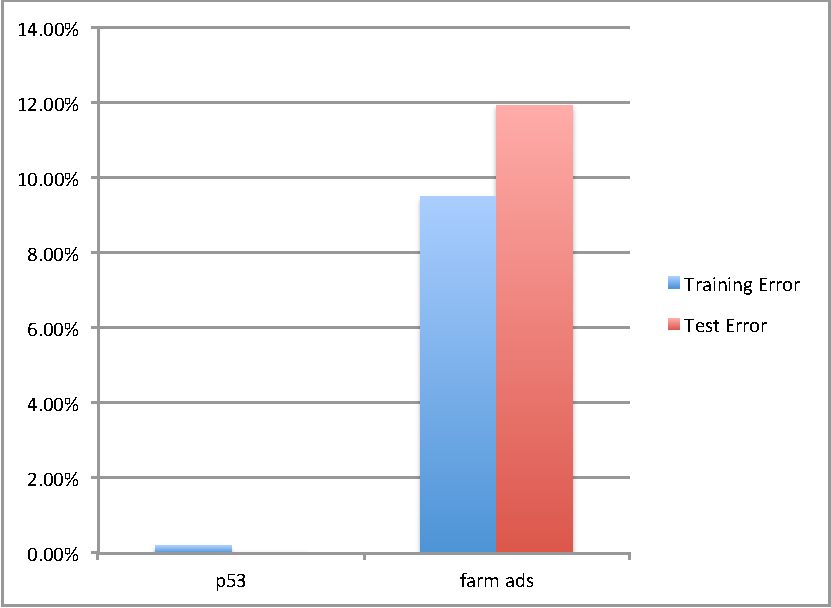
\includegraphics[height=5.0cm]{../../results/classificaiton_errors.pdf}
%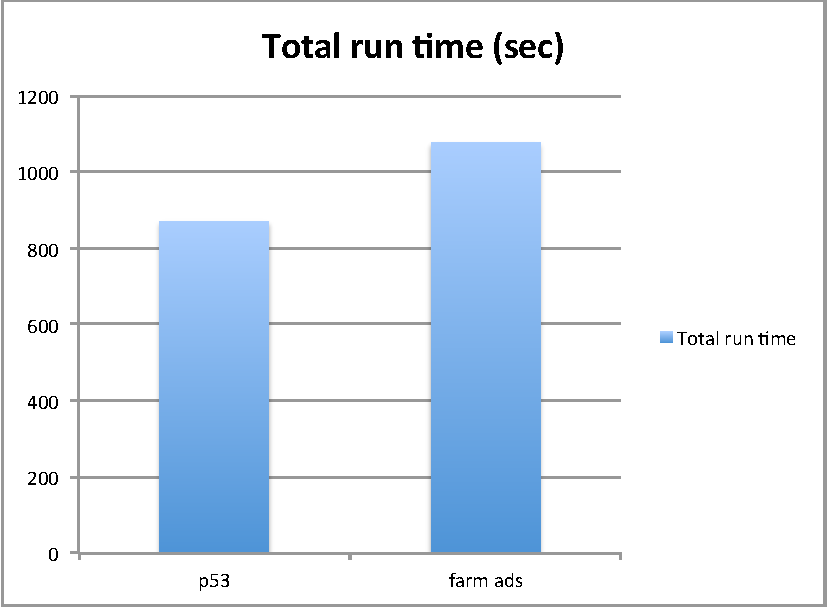
\includegraphics[height=5.0cm]{../../results/runtime.pdf}
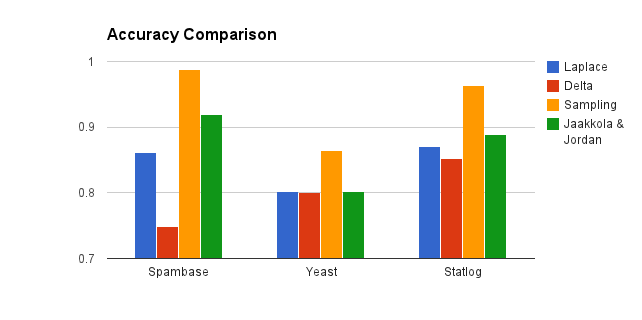
\includegraphics[height=5.0cm]{results/accuracy_comp.png}
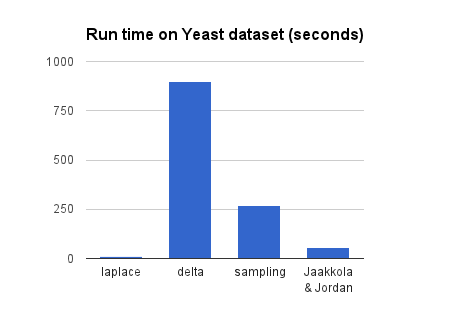
\includegraphics[height=5.0cm]{results/speed_comp.png}

\caption{\small Experiment results; {\bf Top:} Classification accuracy of all algorithms on
four datasets. {\bf Bottom:} Training time for each algorithm on Yeast dataset. }

\label{graphlab}
\end{figure}

\subsubsection{MCMC based estimation}
Our MCMC sampling strategy that we described in section~\ref{sec:MCMCmethod}
converges. Figure~\ref{fig:MCMCconverge} is a plot of the iterations of the Markov 
chain for estimation on a subset of Farms Ads dataset. This is for MLE
estimation without any priors. The X-axix of the figure represents the number of
iteration in sampling and Y-axi si the loglikelihood of theregression model We
also achieve a training accuracy of 8.57\% and a test accuracy of 9.12\% over 
this subset of datset. 

We were only able to run the experiments on this subset of the dataset as the
sampler if slow since we have a rejection sampling component besides various
other samplers. The acceptance ratio of the rejection step is is one quarter on
an average accross number of iterations. In future we plan to fins a better
alternative to this rejection sampler to achieve better speed. 

\begin{figure}[hbt]
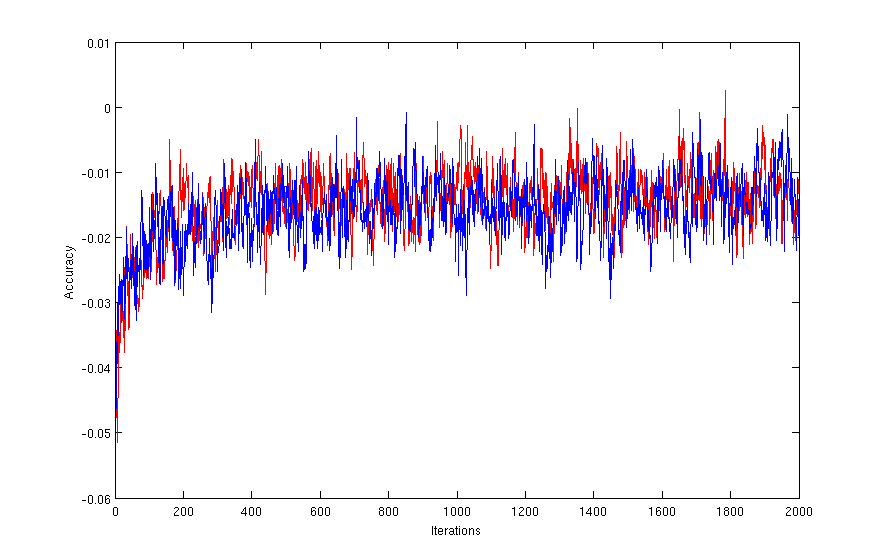
\includegraphics[width=1\textwidth]{results/KSsampleChain.png}
\caption{Two Markov chains (red and blue) converge on the same set of
parameters on the spambase dataset. The
X-axis is the number of iterations and Y-axis is the loglikelihood.}
\label{fig:MCMCconverge}
\end{figure}
